\section{The Prototype Calorimeter}


\subsection{Introduction}
Tungsten Powder/Scintillating Fiber Calorimetry is a novel JLab technology that was originally proposed at the very beginning of the 12 GeV Energy Upgrade project in 1999. This original proposal was to develop a compact calorimeter with good energy resolution and angular resolution at polar angles $\vartheta$$>$35\degree for the CLAS12 spectrometer to fit inside the Central Detector \cite{Cardman2001}. This technique was also considered by calorimetry for the ACCESS mission to the International Space Station to measure intermediate-energy primary cosmic rays. That experiment was interested in a compact calorimeter 
\cite{Access}.
The Tungsten Powder calorimeter’s essential features are compactness, no air gaps between fibers and radiator, homogeneity, simplicity, and unique readout capabilities not otherwise available. From the original proposal there exists a prototype calorimeter designed and built at JLab in 2002. Utilizing unique Tungsten Powder Calorimetry expertise developed at JLab while building of the original prototype can be helpful in further R\&D of the technology.

\subsection{Current Status}

The 12-channel prototype Tungsten Powder calorimeter (see Figure \ref{fig:CalorimeterCasing} and Figure \ref{fig:Prototype}) was designed and built in 2002. The prototype is fully operational and has been preliminarily tested with cosmic rays. The cosmic ray test setup is also available. Dimensions of the active volume filled with Tungsten powder are $L \times W \times H = 4.06" \times 4.06" \times 2.70"$. All structural parts are made of Aluminum alloy. The main constraints that determine the basic parameters for the prototype calorimeter were due to the compact structure of the Central Detector incorporated in the Superconducting Solenoid. On the other hand the calorimeter must provide reasonable energy and spatial resolution. The typical energies of decay photons produced under large angles at 12 GeV are of $E_{\gamma}\sim1$GeV. To provide a sufficiently high absorption power to contain most of the shower generated under angles of $\sim90\degree$ by such photons 10 -- 11 radiation lengths are required. This leads to a radial space of $\sim$10 cm if the materials with properties close to those of Lead Tungstate (8.28 g/cm$^3$) are used. Direct calculations show that in order to provide sufficient mass resolution $\delta m\sim1/3\cdot(m/2)$ for $\pi\degree$ and $\eta$ mesons at the aforementioned momenta it is reasonable to have energy resolution of the order of $\sigma/E_{\gamma}\sim(6-7)\%$ at $E_{\gamma}\sim1$GeV. To detect $\pi\degree$-mesons of lowest energy, the calorimeter must have an energy threshold of $\leq50$MeV.

\begin{figure*}[h]
\centering
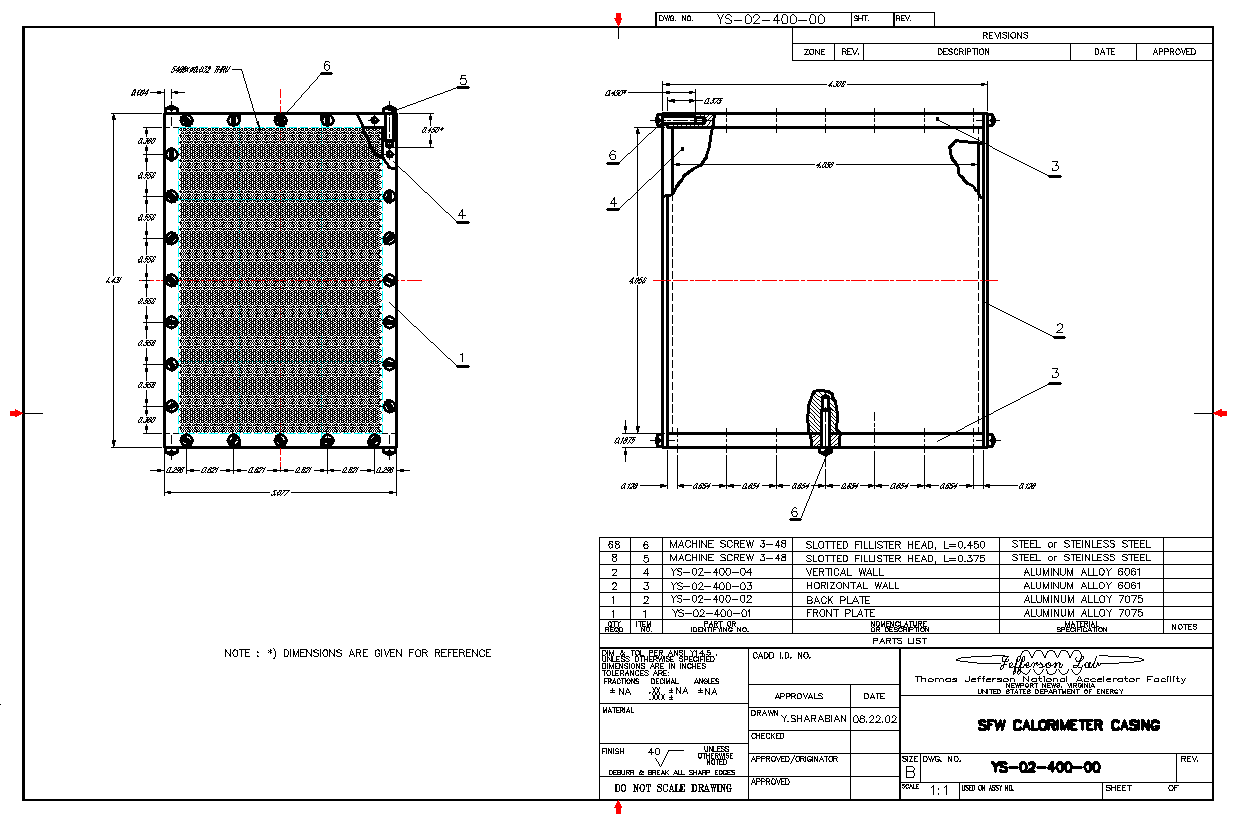
\includegraphics[width=0.975\textwidth]{images/Fig1_CalorimeterCasing.png}
\caption{Calorimeter casing. Side walls have several thousand holes for fibers.}
\label{fig:CalorimeterCasing}
\end{figure*}

\begin{figure}[h]
\centering
\includegraphics[width=0.9\linewidth]{images/Fig2_Prototype_Text.png}
\caption{Prototype Tungsten Powder/Scintillating Fiber calorimeter}
\label{fig:Prototype}
\end{figure}

\begin{figure}[h]
\centering
\includegraphics[width=0.9\linewidth]{images/Fig3_ActiveVolumeCasing_Text.png}
\caption{Active volume casing. Perforated area of $L \times H = 4" \times 2.626"$}
\label{fig:ActiveVolumeCasing}
\end{figure}

\begin{comment}
\begin{figure*}[h] 
  \begin{minipage}[b]{0.5\linewidth}
    \centering
    \includegraphics[width=.85\linewidth]{Fig2_Prototype_Text.png}
    \caption{Prototype Tungsten Powder/Scintillating Fiber calorimeter}
    \label{fig:Prototype}
    %\vspace{4ex}
  \end{minipage}%%
  \begin{minipage}[b]{0.5\linewidth}
    \centering
    \includegraphics[width=.85\linewidth]{Fig3_ActiveVolumeCasing_Text.png}
    \caption{Active volume casing. Perforated area of $L \times H = 4" \times 2.626$}
    \label{fig:ActiveVolumeCasing}
    %\vspace{4ex}
  \end{minipage} 
\end{figure*}
\end{comment}


\subsection{Topology and Geometry}

\begin{figure}[h]
\centering
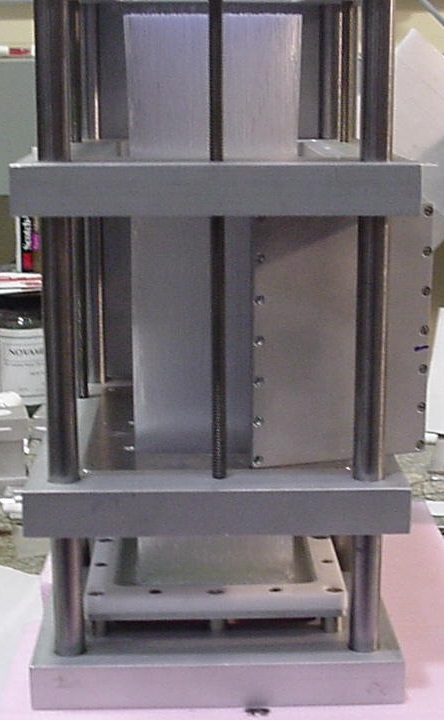
\includegraphics[width=0.65\linewidth]{images/Fig4_InstallFibers_Crop.jpg} 
    \caption{Installation of scintillating fibers in the active volume.} 
    \label{fig:InstallFibers}
\end{figure}

\begin{figure}[h]
\centering
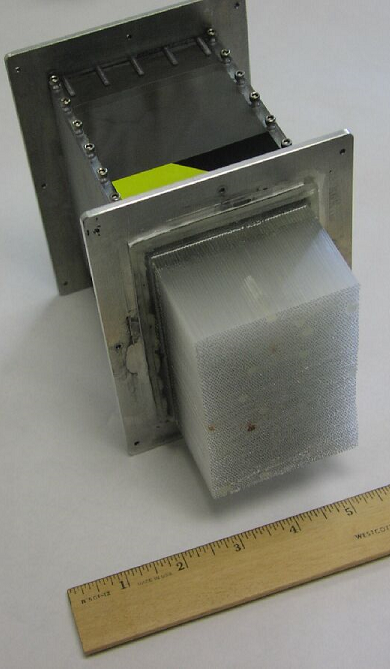
\includegraphics[width=0.65\linewidth]{images/Fig5_CompleteAssemble_Resize.png} 
    \caption{Completely assembled active volume. Fibers are shown before grouping them in bundles (see Figure \ref{fig:FiberBundle}).} 
    \label{fig:CompleteAssemble}
\end{figure}

The overall dimensions of the Prototype are $L \times W \times H = 24.5" \times 4.4" \times 6"$. Dense Tungsten metal powder is used as radiator. Main parts of the active volume casing (see Figure \ref{fig:ActiveVolumeCasing}) are precision perforated plates to hold fibers. There are $98 \times 56 = 5488$ holes total of diameter 0.030" on the each holding plate. The fibers (Bicron BCF-12, $\oslash$ 0.75 mm) make up 35\% of the volume. The plates are precisely aligned relative to each other so that fibers could move freely through the two plates. That required rejection of fibers due to non-uniform thickness along the entire length. All fibers have been installed aligned parallel each other and fixed in place. So while the volume was filled with loose Tungsten powder the fibers would not move and provide maximal homogeneity of the final assembly (see Figure \ref{fig:InstallFibers} and Figure \ref{fig:CompleteAssemble}).

\begin{figure}[h]
\centering
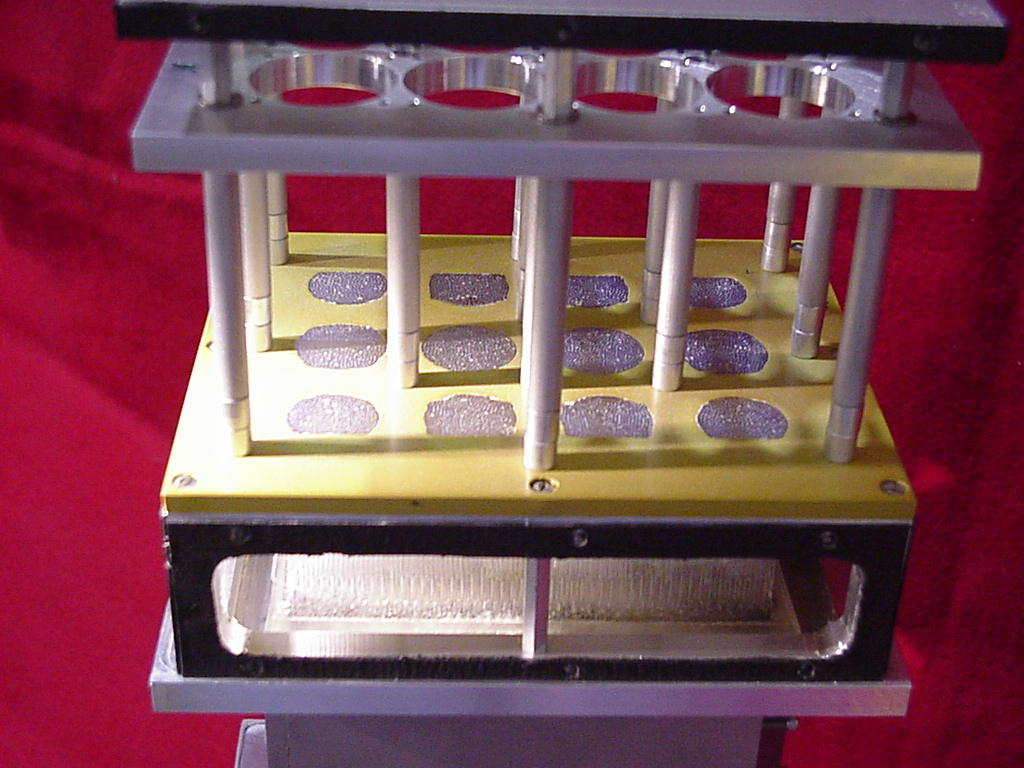
\includegraphics[width=0.9\linewidth]{images/Fig6a_FiberBundle.jpg} 
    \caption{5,488 scintillating fibers bundled up, cut flush and polished.} 
    \label{fig:FiberBundle}
\end{figure}

\begin{figure}[h]
\centering
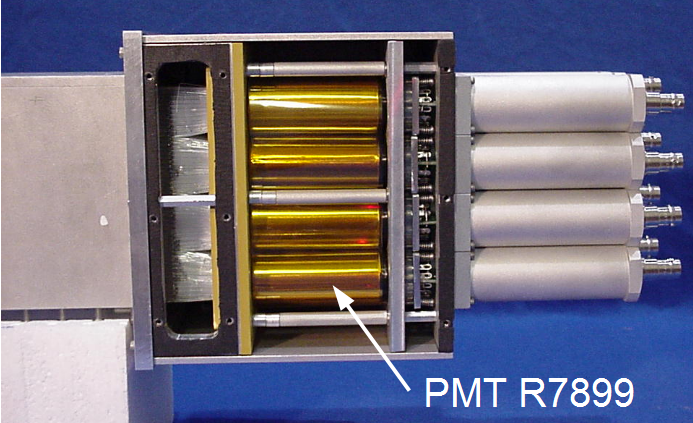
\includegraphics[width=0.9\linewidth]{images/Fig6b_DirectCouplePhototube_Text.png} 
    \caption{Direct coupling of phototubes to bundled up scintillating fibers.} 
    \label{fig:DirectCouplePhototube}
\end{figure}

The fibers are read out from both ends. On one side they are bundled up to form 12 bundles that are cut flush, polished (see Figure \ref{fig:FiberBundle}) and then coupled to the 12 phototubes, Figure \ref{fig:DirectCouplePhototube}.

\begin{figure}[h]
\centering
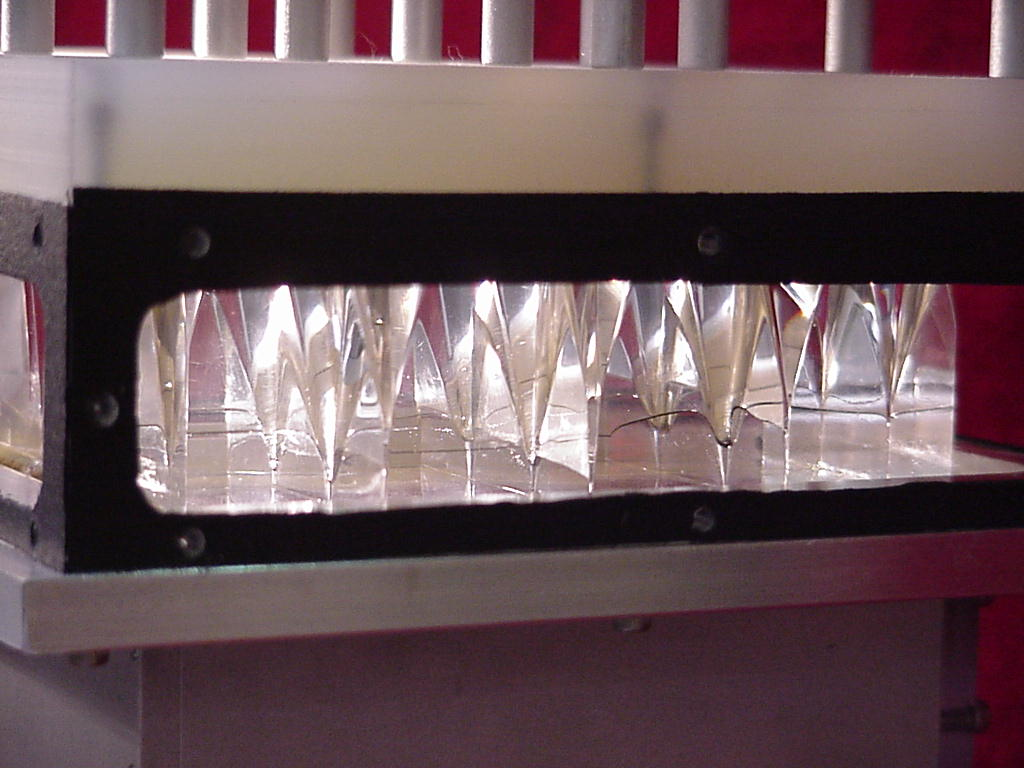
\includegraphics[width=0.9\linewidth]{images/Fig7_AcryllicGuides.jpg} 
    \caption{12 Acrylic light guides glued to the surface formed by polished ends of 5,488 scintillating fibers cut flush} 
    \label{fig:AcryllicGuides}
\end{figure}

\begin{figure}[h]
\centering
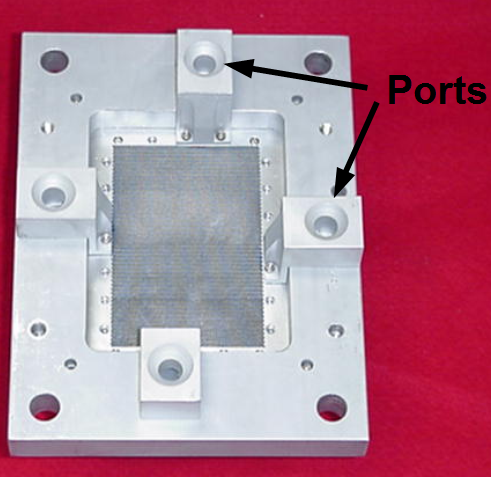
\includegraphics[width=0.9\linewidth]{images/Fig8_Ports_Text.png} 
    \caption{Ports attached to the top of the calorimeter to pour the powder.} 
    \label{fig:Ports}
\end{figure}

From the opposite side the fibers were cut flush and form a flat surface to which after polishing 12 Acrylic light guides are glued (see Figure \ref{fig:AcryllicGuides}) to transmit light from fibers to another set of 12 photomultiplier tubes.

\begin{figure}[h]
\centering
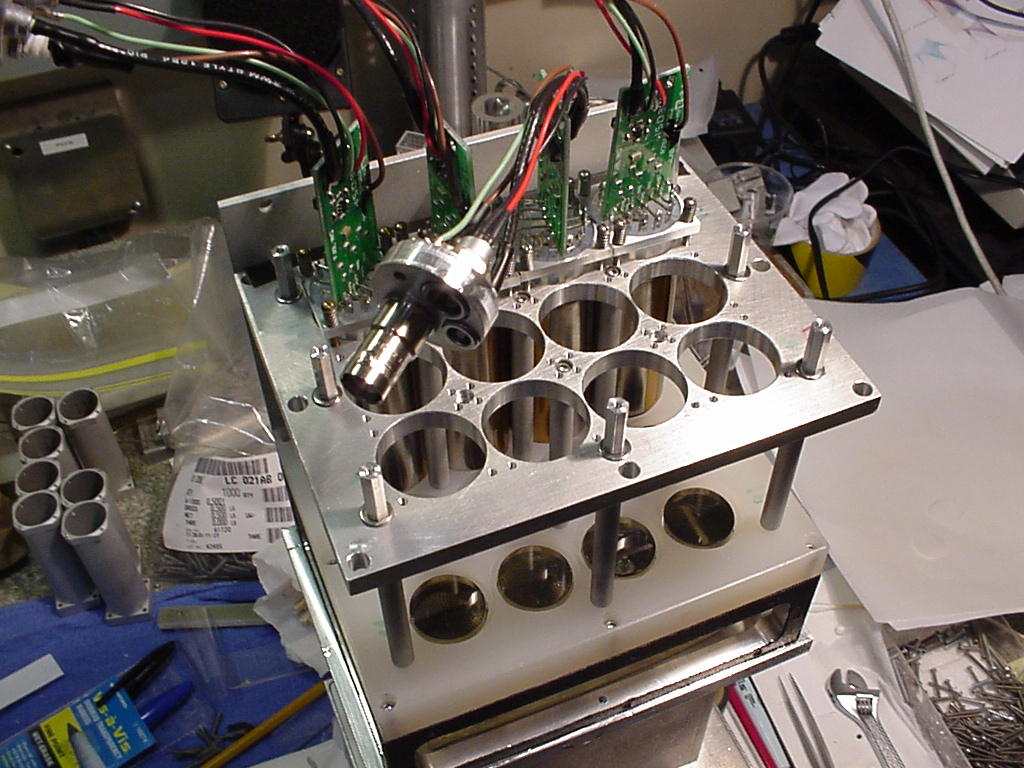
\includegraphics[width=0.9\linewidth]{images/Fig9_InstallPMTs.jpg}
\caption{Installation of PMTs. Cylinders on the left are to hold HV dividers}
\label{fig:InstallPMTs}
\end{figure}

The fibers on both sides are grouped equally to allow for a direct comparison of reliability and performance between the two different light collection couplings, to choose the better performing one. The Tungsten powder is poured into the volume through four temporary ports (Figure \ref{fig:Ports}) on one side.

The powder flow was almost parallel to the fibers axis in order to avoid bending of fibers while the volume is being filled. Final density of the Tungsten powder radiator is about \textbf{12.05 g/cm$^3$} or as compared with density of bulk lead is higher by about 6\%. Installation of the first several photomultiplier tubes with dividers and connectors are shown in Figure \ref{fig:InstallPMTs}. We have used Hamamatsu R7899 1 inch photomultiplier tubes. HV dividers have integrated in them fast preamplifiers providing two identical signals. The overall total density of the prototype active volume is $\sim$8.03 g/cm$^3$.

\subsection{Performance}

To estimate the expected energy resolution one can use shower parameterizations based on simulations and previous calorimeter data \cite{wigmans2000calorimetry}. We require at least 98\% of the electromagnetic shower at energy 1 GeV to be absorbed in calorimeter. The corresponding length of calorimeter is parameterized as Equation \ref{eq:1}:
\begin{equation} \label{eq:1}
    L = 2.5\left[ \log \left( \frac{E_{\gamma}}{\varepsilon} \right) + 1.2 \right]
\end{equation}

where $L$ is the length (measured in radiation lengths), $E_{\gamma}$ is the energy of the incoming photon and $\varepsilon$ is the critical energy of the material:

\begin{equation}
    \varepsilon = y\varepsilon_{sci} + (1-y)\varepsilon_{powder}
\end{equation}

Parameter $y$ is the fraction of plastic fibers in the active volume of honeycomb structure and defined as:

\begin{equation}
    y = \frac{\pi}{2\sqrt{3}}\frac{D^2}{a^2}
\end{equation}

where $D$ is diameter of the fibers and $a$ is distance between them. The material in the calorimeter is a mix of Tungsten powder and Polystyrene scintillating fibers. The radiation length for the mix ($X_0$) that contains a fraction $y$ of scintillating plastic per volume and fraction $(1-y)$ of tungsten powder absorber is obtained using Equation \ref{eq:2}, \cite{Fabjan1985}:

\begin{equation} \label{eq:2}
    \left( \frac{1}{X_0} \right) = \left( \frac{y}{X_{sci}} \right) + \frac{(1-y)}{X_{powder}}
\end{equation}

 where $X_{powder}$ is the radiation length of the loose powder of green density $\rho = \chi \rho_w$, where $\chi < 1$ and $\rho_w$ is the metal Tungsten density. So $X_{powder} = X_w/\chi$, where $X_w =$ 3.5 mm is the radiation length of bulk Tungsten. The length of calorimeter as function of scintillating fibers fraction per active volume at three different radiator densities is shown in Figure \ref{fig:InstallPMTs} where the Prototype radiator density is 12 g/cm$^3$, i.e. 62\% of the bulk density of tungsten. We have investigated what would be the highest reachable density of the compressed tungsten powders of different grades without sintering. The obtained results have shown that the limit is at least 16.37g/cm$^3$ or 85\% of the bulk density of tungsten. The results displayed in Figure \ref{fig:Length} show that at 85\% of radiator density and at the 35\% plastic fiber fraction the calorimeter would be about 6 cm of length and still will provide energy resolution as high as what the prototype can have. In the case that most of the energy at 1 GeV is absorbed in the calorimeter the corresponding errors of the energy measurements are largely defined by \textbf{sampling errors} that are given by Equation \ref{eq:3}:
 
 \begin{equation} \label{eq:3}
     \left( \frac{\sigma}{E} \right)_{samp} = \frac{0.027}{\sqrt{E}}\sqrt{\frac{D}{F_{samp}}}
 \end{equation}
 
 where the sampling fraction $F_{samp}$ is defined as Equation \ref{eq:4}:
 
 \begin{equation} \label{eq:4}
     F_{samp} = \frac{ V_{acryl} \left( \dv{E}{x} \right)_{MIP}^{acryl} }{ V_{acryl} \left( \dv{E}{x} \right)_{MIP}^{acryl} + V_{powder} \left( \dv{E}{x} \right)_{MIP}^{powder} }
 \end{equation}
 
 Relative energy resolution is plotted as function of plastic fiber fraction in the active volume for four different diameters of fibers is shown in Figure \ref{fig:RelNrg}. For the prototype, i.e. at 35\% of plastic fraction and fibers diameter of 0.75 mm (0.030") one can expect to get the resolution ~6.5\%. At fixed plastic fraction it is possible to improve the resolution by using fibers of smaller diameter due to higher homogeneity of the assembly.
 
\begin{figure}[h]
\centering
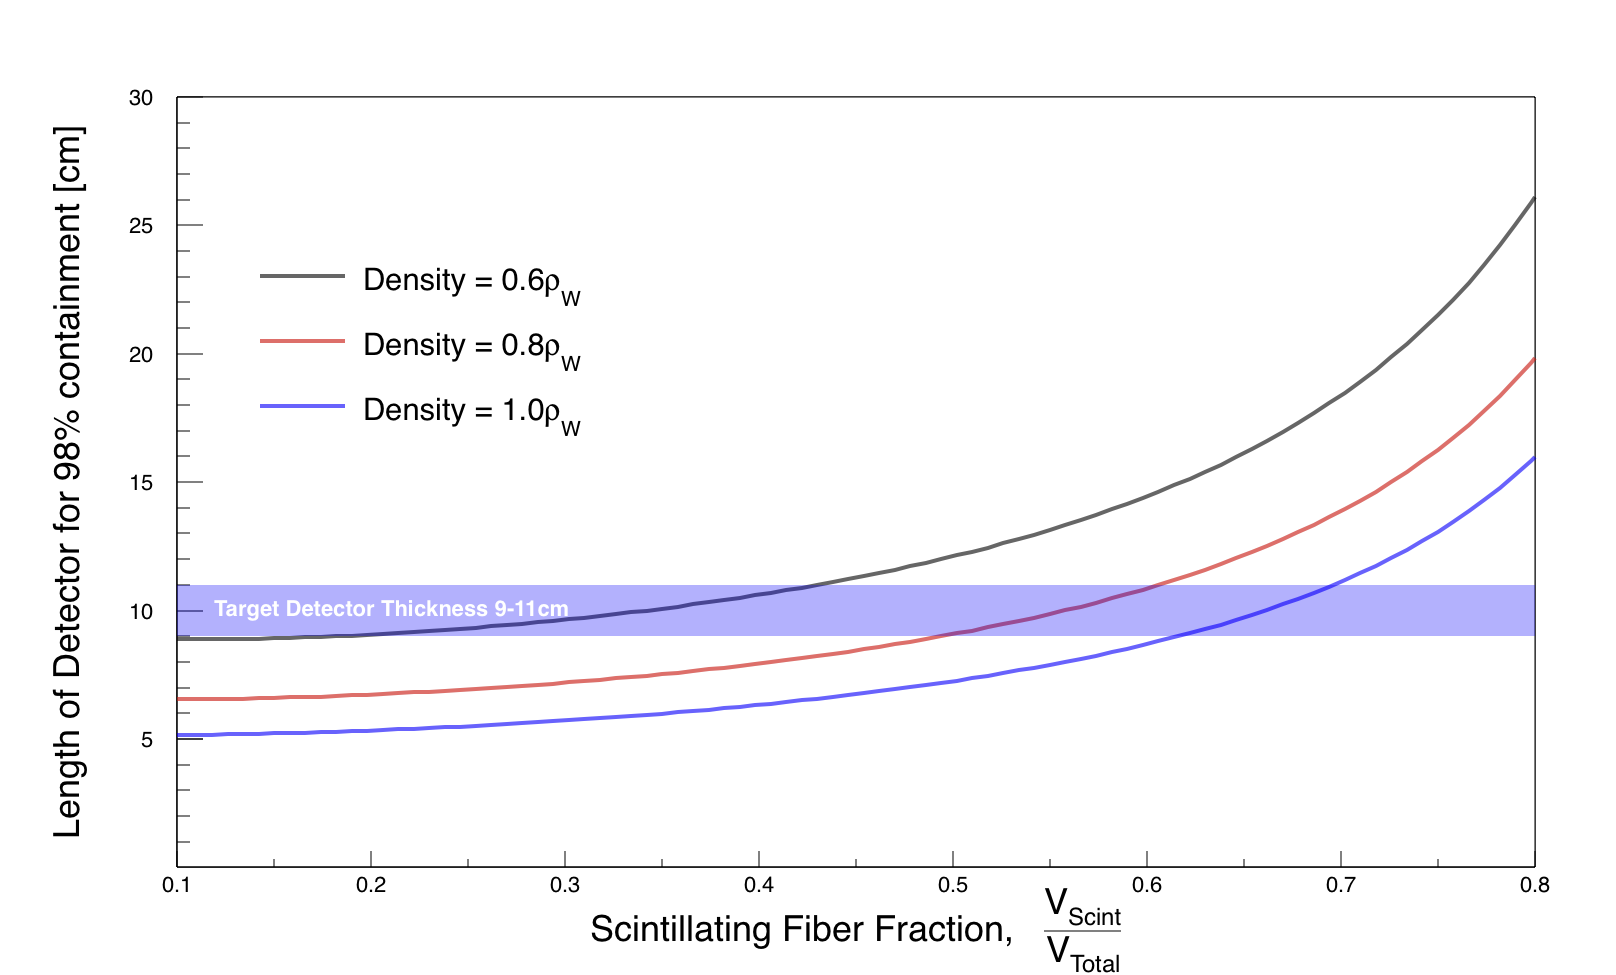
\includegraphics[width=0.95\linewidth]{images/Fig10_Length.png}
\caption{Length of calorimeter absorbing 98\% energy of incident particle versus fiber fraction per volume of the calorimeter. The curves are for different absorber densities and 1 GeV incident photons.}
\label{fig:Length}
\end{figure}

\begin{figure}[h]
\centering
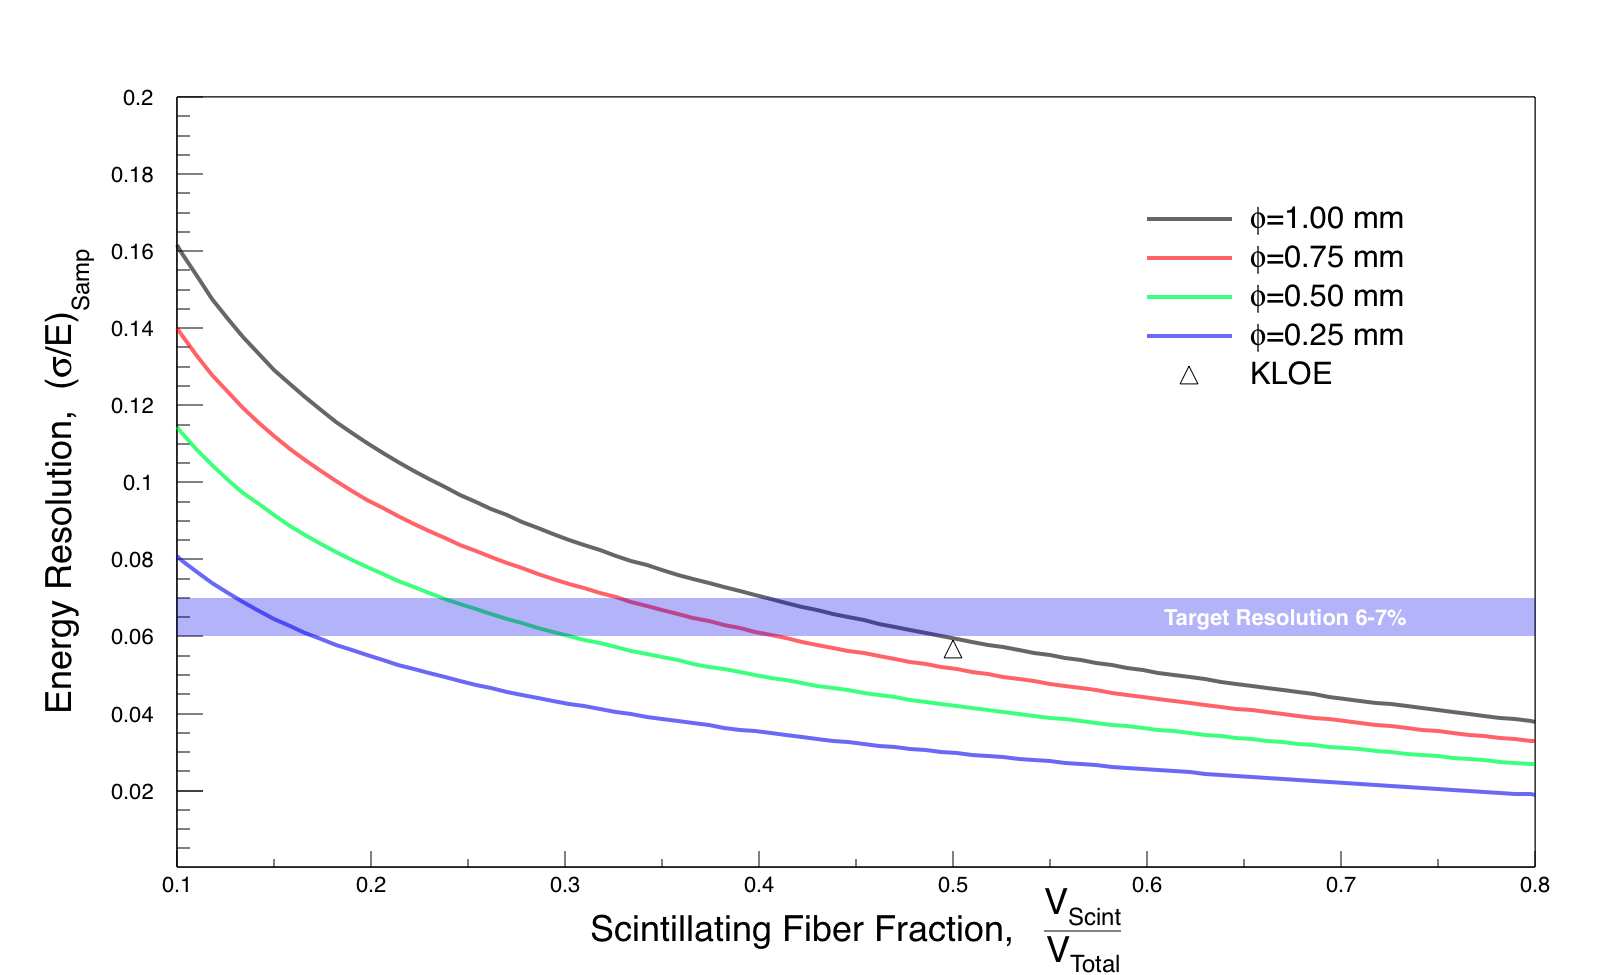
\includegraphics[width=0.95\linewidth]{images/Fig11_RelNrg.png}
\caption{Relative energy resolution versus fiber fraction per volume in the calorimeter. The curves are for 1 GeV incident photons. The resolution obtained by the KLOE Collaboration \cite{Antonelli1995} at Frascatti with a sampling calorimeter (50\% of plastic fraction) using lead (Pb) absorber and 1 mm fibers is shown as well ($\Delta$).}
\label{fig:RelNrg}
\end{figure}

Major general advantages of the proposed calorimeters are possibilities of:

\begin{itemize}
    \item Using fibers of much smaller diameter keeping overall dimensions of the active volume and its density unchanged, i.e. at given plastic fraction and radiator density considerably increasing the homogeneity to improve energy resolution.  (Thinnest  Polystyrene scintillators that can still scintillate are 80 to 120$\mu$m of thickness)
    \item Building more “efficient”, i.e. more compact calorimeters with denser radiator while also improving the energy resolution
    \item Reaching better resolution with fewer number of fibers as compared with traditional sampling calorimeters
    \item Great freedom in organizing light collection by installing fibers along different directions, curved and etc. in the same volume providing  2D or 3D or even more complicated measurements (particle ID)
    \item Reducing number of fibers to be read out at given fixed resolution (minimal number is just one fiber to read out)
\end{itemize}